%*****************************************
\chapter{Correlation}\label{cor:correlation}
%*****************************************
%TODO Reviewed

\section{Introduction}

Correlation is a method used to describe relationships between two variables. For example, if some research project plotted the ages of people who started smoking and the family income of those people then a correlation would attempt to determine if there is some relationship between those two factors.

This lab explores both correlation and scatter plots, which are graphic tools designed to make correlations easier to understand. 

\section{Correlation and Causation}

From the outset of this lab, it is important to remember that there is a huge difference between correlation and causation. Just because two factors are correlated in some way does not lead to a conclusion that one is causing the other. As an example, if a research project found that students who spend more hours studying tend to get higher grades this would be an interesting correlation. However, that research, by itself, could not prove that longer studying hours causes higher grades. There could be other intervening factors that are not accounted for in this simple correlation (like the type of final examination used). As an egregious example to prove this point, consider that the mean age in the United States is rising (that is, people are living longer; thus, there are more elderly people in the population) and that human trafficking crime is increasing. While these two facts may be correlated, it would not follow that old people are responsible for human trafficking! Instead, there are numerous social forces in play that are not accounted for in this simple correlation. It is important to keep in mind that correlation does not equal causation as you read research.

\subsection{Pearson's R}\label{cor:pearsons_r}

Pearson's Product-Moment Correlation Coefficient (normally called \textit{Pearson's r}) is a measure of the strength of the relationship between two variables. Pearson's r is a number between $ -1.0 $ and $ +1.0 $, where $ 0.0 $ means there is no correlation between the two variables and either $ +1.0 $ or $ -1.0 $ means there is a perfect correlation. A positive correlation means that as one variable increases the other also increases. For example, as people age they tend to weigh more so a positive correlation would be expected between age and weight. A negative correlation, on the other hand, means that as one variable increases the other decreases. For example, as people age they tend to run slower so a negative correlation would be expected between age and running speed. In general, both the strength and direction of a correlation is indicated by the value of ``r'':

\rowcolors{1}{gray!25}{}
\begin{center}
  \begin{tabular}{ll}
    \hline 
    \textbf{Correlation} & \textbf{Description}  \\ 
    \hline 
    $ +.70 $ or higher & Very strong positive  \\ 
    $ +.40 $ to $ +.69 $ & Stong positive \\ 
    $ +.30 $ to $ +.39 $ & Moderate positive \\ 
    $ +.20 $ to $ +.29 $ & Weak positive \\ 
    $ +.19 $ to $ -.19 $ & No or negligible \\ 
    $ -.20 $ to $ -.29 $ & Weak negative \\ 
    $ -.30 $ to $ -.39 $ & Moderate negative \\ 
    $ -.40 $ to $ -.69 $ & Strong negative \\ 
    $ -.70 $ or less & Very strong negative \\ 
    \hline 
  \end{tabular} 
\end{center}

As an example from the \textit{bdims} dataset, the correlation between weight and waist girth (Wgt - Wai.Gi) is $ +0.904 $ so there is a very strong positive correlation between these two factors. This would be expected since people who weigh more would be expected to have larger waists. Here are a few other correlations from the \textit{dbims} dataset:

\rowcolors{1}{gray!25}{}
\begin{center}
  \begin{tabular}{lcl}
    \hline 
    \textbf{Variables} & \textbf{Correlation} & \textbf{Description}  \\ 
    \hline 
    Weight\textemdash Waist Girth & $ 0.904 $ & Very Strong Positive  \\ 
    Weight\textemdash Ankle Diameter & $ 0.726 $ & Very Strong Positive  \\ 
    Height\textemdash Chest Depth  & $ 0.553 $ & Strong Positive  \\ 
    Height\textemdash Hip Girth & $ 0.339 $ & Moderate Positive  \\ 
    Height\textemdash Thigh Girth & $ 0.116 $ & No Correlation  \\ 
    \hline 
  \end{tabular}
  \label{cor:table01} 
\end{center}

\subsection{Spearman's Rho}\label{cor:spearmans_rho}

Pearson's r is only useful if both data elements being correlated are interval or ratio in nature. When the one or both data elements are ordinal or nominal then a statistically different process must be used to calculate a correlation, and that process is \textit{Spearman's Rho}. Other than the process used to calculate Spearman's Rho, the concept is exactly the same as for Pearson's r and the result is a correlation between $ -1 $ and $ +1 $ where the strength and direction of the correlation is determined by its value.

For example, imagine that a dataset included information about the age of people who purchased various makes of automobiles. Since the ``makes'' would be selected from a list (Ford, Chevrolet, Honda, etc.), Spearman's Rho would be used to calculate the correlation between the customers' preference for the make of an automobile and their age. Perhaps the correlation would come out to $ +0.534 $ (this is just a made-up number). This would indicate that there was a strong positive correlation between these two variables; that is, people tend to prefer a specific make based upon their age; or, to put it another way, as people age their preference for automobile make changes in a predictable way.

Pearson’s r and Spearman's Rho both calculate correlation and it is reasonable to wonder which method should be used in any given situation. A good rule of thumb is to use Pearson's r if both data items being correlated are interval or ratio and use Spearman's rho if one or both are ordinal or nominal. Imagine a series of survey questions that permitted people to select from only a small group of possible answers. As an example, perhaps respondents are asked to select one of five responses ranging from ``Strongly Agree'' to ``Strongly Disagree'' for statements like ``I enjoyed the movie.'' Restricting responses to only one of five options creates ordinal data and to determine how well the responses to these questions correlate with something like the respondents' ages, Spearman's Rho would be an appropriate choice.

As an example from the \textit{email} dataset, the correlation between Image and CC is $ +0.808 $ so there is a very strong positive correlation between these two factors. Here are a few other correlations from the \textit{email} dataset, all using Spearman's Rho:

\rowcolors{1}{gray!25}{}
\begin{center}
  \begin{tabular}{lcl}
    \hline 
    \textbf{Variables} & \textbf{Correlation} & \textbf{Description}  \\ 
    \hline 
    Image\textemdash Exclaim\_Mess & $ 0.522 $ & Strong Positive  \\ 
    Image\textemdash Line\_Breaks & $ 0.491 $ & Strong Positive  \\ 
    Image\textemdash Attach  & $ 0.927 $ & Very Strong Positive  \\ 
    Line\_Breaks\textemdash Dollar & $ 0.453 $ & Strong Positive  \\ 
    Exclaim\_Mess\textemdash CC & $ 0.408 $ & Strong Positive  \\ 
    \hline 
  \end{tabular}
  \label{cor:table02} 
\end{center} 

\section{Significance} \label{cor:significance}

Most people use the word ``significant'' to mean ``important'' but researchers and statisticians have a much different meaning for ``significant'' and it is vital to keep that difference in mind.

In statistics and research, ``significance'' means that the experimental results were such that they would not likely have been produced by mere chance. For example, if a coin is flipped $ 100 $ times, heads should come up $ 50 $ times. Of course, by pure chance, it would be possible for heads to come up $ 55 $ or even $ 60 $ times. However, if heads came up $ 100 $ times, researchers would suspect that something unusual was happening (and they would be right!). To a researcher, the central question of significance is ``How many times can heads come up and still be considered just pure chance?'' That number is the statistical significance level. 

In general, researchers use one of three significance levels: $ 1\% $, $ 5\% $, or $ 10\% $. A researcher conducting The Great Coin-Tossing Experiment may start by simply stating ``This result will be significant at the $ 5\% $ level.'' That would mean that if the coin were tossed $ 100 $ times, then anything between $ 47.5-52.5 $ (a 5\% spread) ``heads'' tosses would be merely chance. However, $ 47 $ or $ 53 $ ``heads'' would be outside that $ 5\% $ spread and would be significant. 

It must seem somewhat subjective for a researcher to simply select the desired significance level, but most researchers in business and the social and behavioral sciences (like education, sociology, and psychology) tend to choose a significance level of $ 5\% $.\footnote{The reason that $ 5\% $ is usually selected as a significance level can be traced back to R.A. Fisher who published a book in $ 1925 $ that included statistical tables for researchers. His work was profoundly influential and values in the $ 5\% $ table became the most commonly cited levels in published research for many decades.} There is no real reason for choosing that level today other than it is just the way things have traditionally been done for many years. Therefore, if a researcher selected something other than $ 5\% $, peer researchers would want some explanation concerning the ``weird'' significance level.

Keep in mind, though, that statistical significance is not the same as practical significance. \textit{Wikipedia}, that great repository of knowledge, includes this interesting example\footnote{\url{http://en.wikipedia.org/wiki/Statistical\_significance}}: 

\bigskip
\hfill\begin{minipage}{\dimexpr\textwidth-1cm}
As used in statistics, significant does not mean important or meaningful, as it does in everyday speech. For example, a study that included tens of thousands of participants might be able to say with great confidence that residents of one city were more intelligent than people of another city by $ 1/20 $ of an IQ point. This result would be statistically significant, but the difference is small enough to be utterly unimportant.
\end{minipage}
\bigskip

\subsection{Chi-Square}\label{cor:chi_square}

One of the most common measurements of statistical significance is the chi-square test, but this test should only be used if both variables are nominal. The basic idea behind this test is to determine what values would be expected by chance and compare that to the values actually obtained by experiment. The formula for a chi-square test is somewhat complex but \texttt{SOFA} handles chi-square calculations without any problem at all. The following chi-square values were obtained from the \textit{email} dataset:

\rowcolors{1}{gray!25}{}
\begin{center}
  \begin{tabular}{lc}
    \hline
    \textbf{Variables} & \textbf{Chi-Square} \\ 
    \hline 
    Spam\textemdash Exclaim\_Subj & $ 0.256 $ \\ 
    Spam\textemdash Image & $ 5.927 $ \\ 
    Spam\textemdash Urgent\_Subj & $ 15.374 $ \\ 
    Spam\textemdash Attach & $ 104.825 $ \\ 
  \end{tabular} 
\end{center}

While it is difficult to decide if any give chi-square statistic is ``good'' or ``bad,'' in general the larger that number then the stronger the relationship between the two variables. In the above table, for example, there would seem to be virtually no relationship between Spam and Exclaim\_Subj but there is a strong relationship between Spam and Attach.

As an aid to determining whether a calculated chi-square is significant, a \textit{p-value} (that stands for ``probability value'') is usually also calculated. A p-value answers the question, ``what is the probability that an observed phenomenon is due to chance?'' For example, the p-value for each of the above chi-square statistics is:

\rowcolors{1}{gray!25}{}
\begin{center}
  \begin{tabular}{lcc}
    \hline
    \textbf{Variables} & \textbf{Chi-Square} & \textbf{P-Value} \\ 
    \hline 
    Spam\textemdash Exclaim\_Subj & $ 0.256 $ & $ 0.6129 $ \\ 
    Spam\textemdash Image & $ 5.927 $ & $ 0.2047 $ \\ 
    Spam\textemdash Urgent\_Subj & $ 15.374 $ & $ 8.820 \times 10^{-5} $ \\ 
    Spam\textemdash Attach & $ 104.825 $ & $ 0.00 $ \\ 
    \hline 
  \end{tabular} 
\end{center}

Notice that as the chi-square statistic gets larger the p-value gets smaller since there is an inverse relationship between those values. In the Significance section above, page \pageref{cor:significance}, the concept of a $ 5\% $ significance level was developed so any p-value smaller than $ 0.05 $ is considered significant; that is, it is not likely due to chance. If the researcher for the ``email'' project was using a $ 5\% $ ($ 0.05 $) significance level then there is no significance in the correlation between spam and exclaim\_subj or spam and image since the p-level for those two correlations is greater than $ 0.05 $. However, the relationship between spam and urgent\_subj and spam and attach is significant since the p-level for those two correlations is smaller than $ 0.05 $.

In short, a significant correlation would have a large chi-square statistic and a small p-level value (less than $ 0.05 $, normally).

\subsection{Degrees of Freedom}\label{cor:degrees_of_freedom}

One other statistic is often evoked when discussing significance: \textit{Degrees of Freedom}. While this statistic can be confusing to understand\footnote{There is an excellent discussion about Degrees of Freedom at \url{http://blog.minitab.com/blog/statistics-and-quality-data-analysis/what-are-degrees-of-freedom-in-statistics}}, it is fairly easy to calculate. Keep in mind that degrees of freedom are only meaningful for nominal or ordinal data and is calculated by determining the number of levels for each of the variables under consideration, subtract one from each of those levels, and multiply the result. As an example, when calculating the ``spam\textemdash Attach'' chi-square, there were two levels for ``spam'' (no/yes) and eight levels for ``attach'' ($ 0, 1, 2, 3, 4, 5, 6, 7 $). Subtracting one from each of those leaves one and seven and then multiplying those two numbers ends with seven degrees of freedom. \texttt{SOFA} displays the degrees of freedom with the chi-square calculation.

Here are a few degrees of freedom from the \textit{email} dataset to help explain this concept. In each case, the number of levels for each variable are in parenthesis following the variable name. 

\rowcolors{1}{gray!25}{}
\begin{center}
  \begin{tabular}{lc}
    \hline
    \textbf{Variables} & \textbf{Degrees of Freedom} \\ 
    \hline 
    Spam (2)\textemdash Exclaim\_Subj (2) & $ (2-1)(2-1)=1 $ \\ 
    Spam (2)\textemdash Image (5) & $ (2-1)(5-1)=4 $ \\ 
    Number (3)\textemdash Image (5) & $ (3-1)(5-1)=8 $ \\ 
    Number (3)\textemdash Attach (8) & $ (3-1)(8-1)=14 $ \\ 
    \hline 
  \end{tabular} 
\end{center}

\section{Scatter Plots}

A scatter plot is a two-dimensional graph of ordered pairs that indicates the relationship between two variables. While a scatter plot could be created from nominal or ordinal data, it is normally only used for interval and ratio data. For example, the correlation between weight and waist girth in the \textit{dbims} dataset was calculated at $ 0.904 $ (see the table on page \pageref{cor:table01}). Figure \ref{cor:weight_waist_scatter_plot} is the scatter plot for that correlation:

\begin{figure}[H]
  \begin{center}
    \fbox{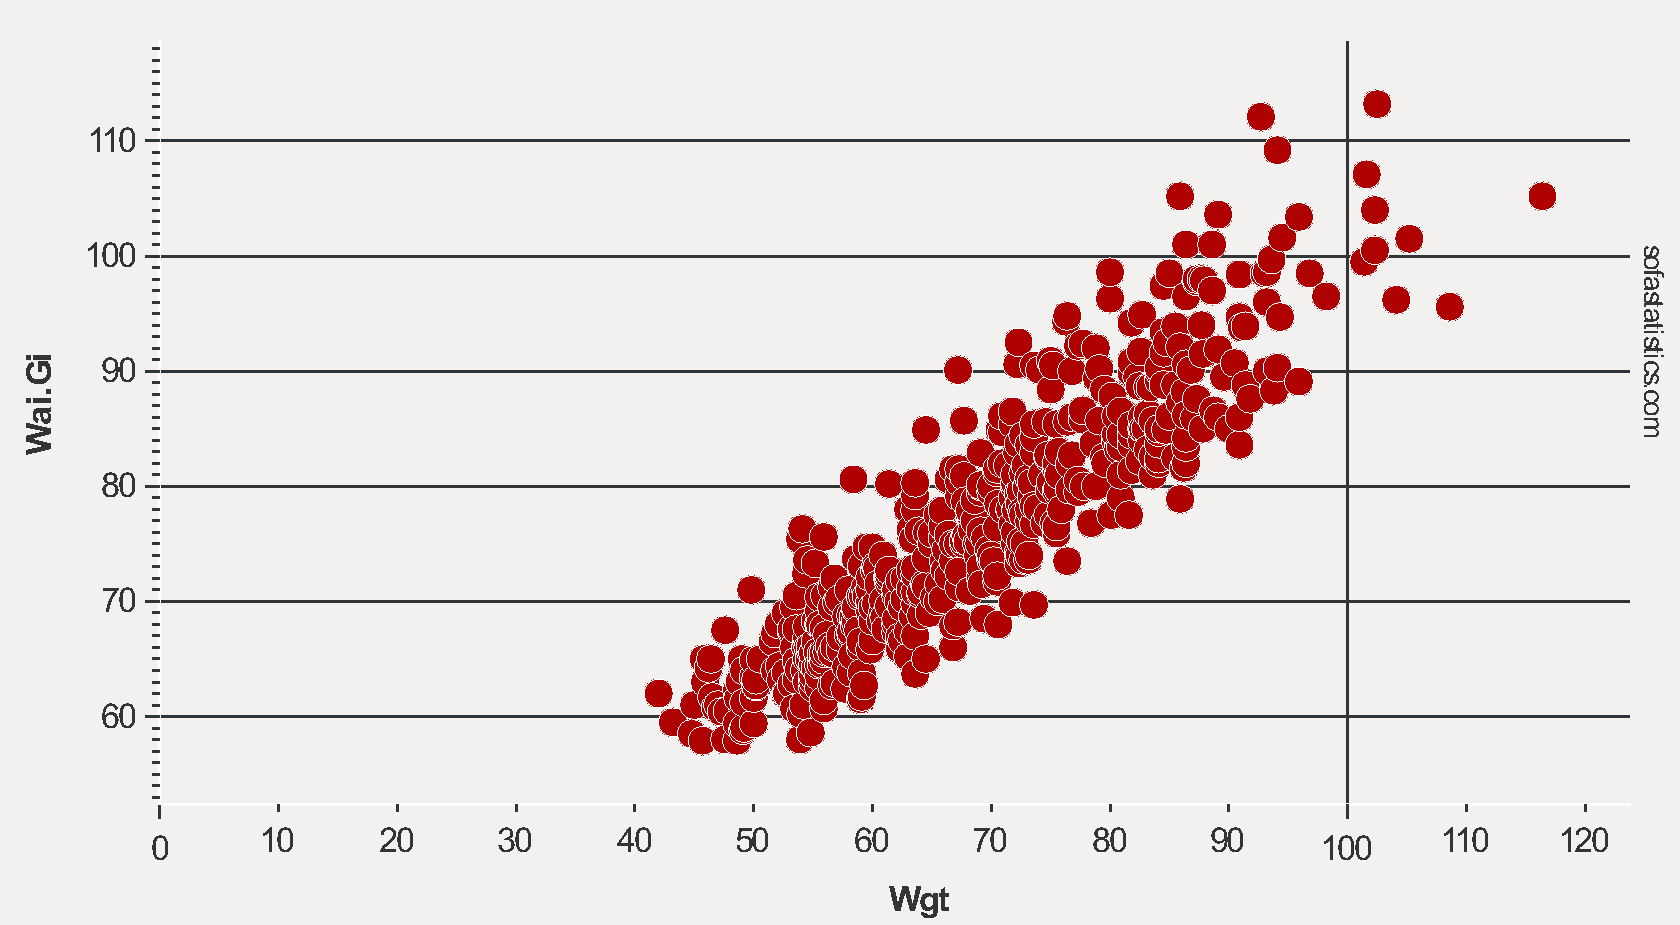
\includegraphics[width=0.95\linewidth]{gfx/cor005}}
    \caption{Weight-Waist Girth}
    \label{cor:weight_waist_scatter_plot}
  \end{center}
\end{figure}

Each of the red dots is a single point in the dataset. For example, the farthest dot to the right is for a weight of $ 116.4 $ and a waist girth of $ 105.2 $ Notice that, generally, as the weight increases (X-Axis) the waist girth also increases (Y-Axis), which indicates a positive correlation. Also notice that the dots are very close together which indicates a strong correlation. Compare this to the next illustration:

\begin{figure}[H]
  \begin{center}
    \fbox{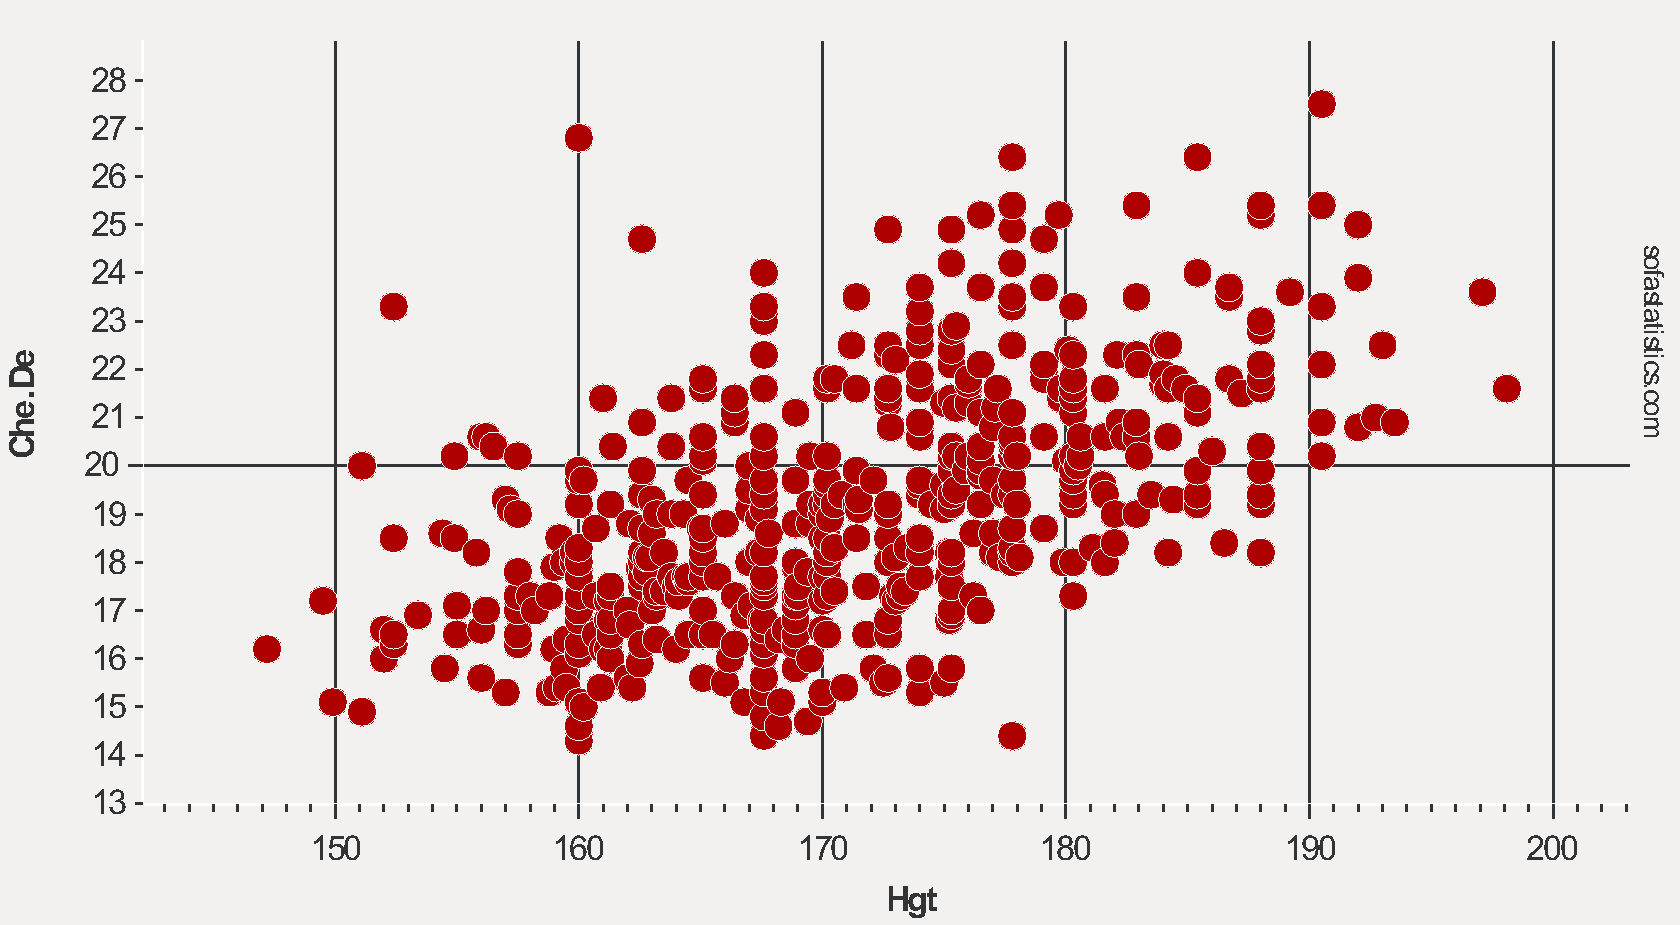
\includegraphics[width=0.95\linewidth]{gfx/cor010}}
    \caption{Height-Chest Depth}
    \label{cor:height_chest_scatter_plot}
  \end{center}
\end{figure}

Figure \ref{cor:height_chest_scatter_plot} is the scatter plot for the correlation between height and chest depth, which was calculated at $ 0.553 $ (see the table on page \pageref{cor:table01}). While there is still a clear upward trend to these dots (a positive correlation), they are more scattered out (a weak correlation). As one final example, consider the scatter plot for height and thigh girth. 

\begin{figure}[H]
  \begin{center}
    \fbox{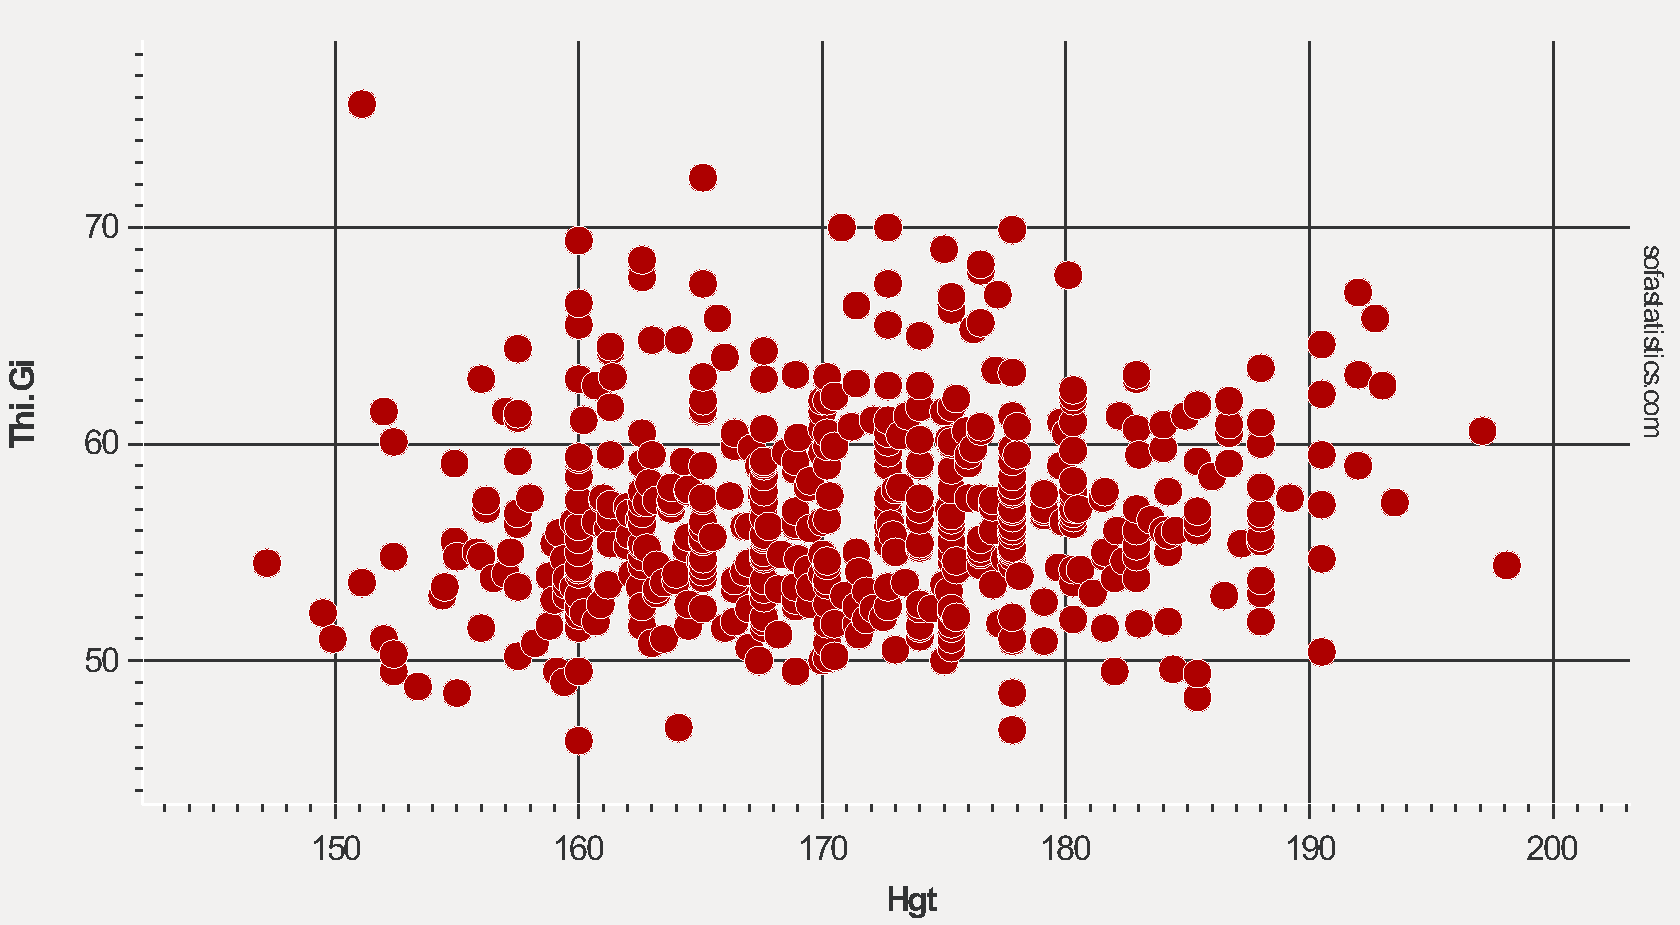
\includegraphics[width=0.95\linewidth]{gfx/cor015}}
    \caption{Height-Thigh Girth}
  \end{center}
\end{figure}

The correlation $ 0.116 $ so there is no clear direction for the plot and the dots are very scattered.

\section{Procedure}

\subsection{Pearson's R}\label{cor:pearsons_r_proc}

Start \texttt{SOFA} and select ``Statistics'' then:

\begin{enumerate}
  \item Select ``Select a Statistical Test Here''
  \item Select ``Correlation - Pearson's''
  \item Click ``Configure Test''

  \begin{figure}[H]
    \begin{center}
      \fbox{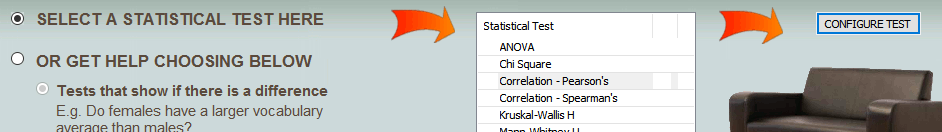
\includegraphics[width=0.95\linewidth]{gfx/cor020}}
      \caption{Starting Pearson's R}
    \end{center}
  \end{figure}

  \item Data Source Table: gifted (It is desired to see if there is a correlation between the age when children first learn to count and the time spent watching cartoons.)
  \item Group A: Count (this is the ``X-Axis'' or independent variable)
  \item Group B: Cartoons (this is the ``Y-Axis'' or dependent variable)

  \begin{figure}[H]
    \begin{center}
      \fbox{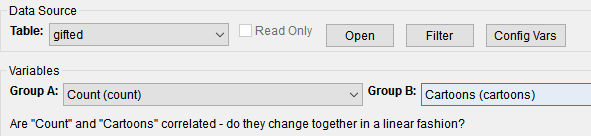
\includegraphics[width=0.95\linewidth]{gfx/cor025}}
      \caption{Calculating Pearson's R for Cartoons-Count}
    \end{center}
  \end{figure}

  \item Click ``Show Results'' and read the results at the bottom of the window. \texttt{SOFA} reports the ``Two-tailed p value'' (described as simply ``p-value'' earlier in this lab document) of $ 0.3670 $, Pearson's R of $ 0.155 $, with $ 34 $ degrees of freedom.

  \begin{figure}[H]
    \begin{center}
      \fbox{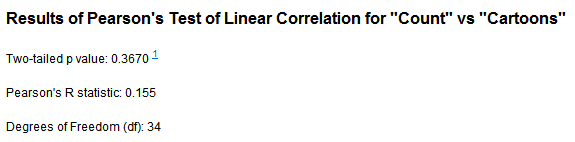
\includegraphics[width=0.95\linewidth]{gfx/cor030}}
      \caption{Pearson's R for Cartoons-Count}
    \end{center}
  \end{figure}

  \item \texttt{SOFA} also displays a scatter plot with a regression line and reports its slope ($ 0.023 $) and Y-Intercept ($ 2.371 $)\footnote{Regression and the use of the slope/intercept information is covered in Lab \ref{reg:regression}, page \pageref{reg:regression}}. 

  \begin{figure}[H]
    \begin{center}
      \fbox{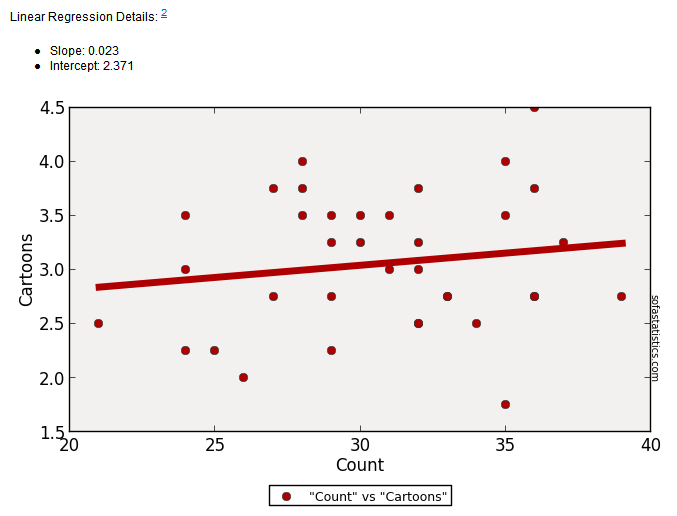
\includegraphics[width=0.95\linewidth]{gfx/cor035}}
      \caption{Scatterplot and Regression Line for Cartoons-Count}
    \end{center}
  \end{figure}

\end{enumerate}

The following table lists the calculated statistics for several Pearson's R correlations from the \textit{gifted} dataset. This could be used for practice in obtaining Pearson's R.

\rowcolors{1}{gray!25}{}
\begin{center}
  \begin{tabular}{lccc}
    \hline 
    \textbf{Variables} & \textbf{P} & \textbf{R} & \textbf{DF} \\ 
    \hline 
    Count-Edutv     & $ 0.2065 $ & $ -0.216 $ & $ 34 $ \\ 
    Read-Score      & $ 1.006 \times 10^{-3} $ & $  0.525 $ & $ 34 $ \\ 
    Motheriq-Read   & $ 0.8032 $ & $ -0.043 $ & $ 34 $ \\ 
    \hline 
  \end{tabular} 
\end{center}

\subsection{Activity 1: Pearson's R} \label{cor:act01}

Using the \textit{maincafe} dataset in \texttt{SOFA}, determine Pearson's R for Length (Group A) and Bill (Group B). Submit a screen capture from \texttt{SOFA} that shows the Two-tailed p value, Pearson's R statistic, Degrees of Freedom, and Linear Regression Details (Slope and Intercept).

\subsection{Spearman's Rho}\label{cor:spearmans_rho_proc}

Start \texttt{SOFA} and select ``Statistics'' then:

\begin{enumerate}
  \item Select ``Select a Statistical Test Here''
  \item Select ``Correlation - Spearmans's''
  \item Click ``Configure Test''
  
  \begin{figure}[H]
    \begin{center}
      \fbox{
\includegraphics[width=0.95\linewidth]{gfx/cor040}}
      \caption{Starting Spearman's Rho}
    \end{center}
  \end{figure}
  
  \item Data Source Table: email (It is desired to see if there is a correlation between the number of attachments to a message and its being identified as spam.)
  \item Group A: Attach (this is the ``X-Axis'' or independent variable)
  \item Group B: Spamnum (this is the ``Y-Axis'' or dependent variable)

  \begin{figure}[H]
  \begin{center}
    \fbox{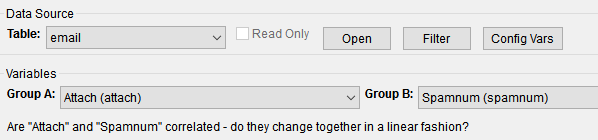
\includegraphics[width=0.95\linewidth]{gfx/cor045}}
    \caption{Setting Up Spearman's Rho}
  \end{center}
  \end{figure}
  
  \item Read the results of calculating Spearman's Rho at the bottom of the window.

  \begin{figure}[H]
    \begin{center}
      \fbox{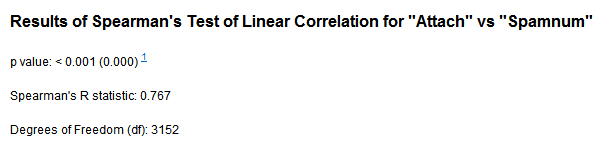
\includegraphics[width=0.95\linewidth]{gfx/cor050}}
      \caption{Spearman's Rho Results}
    \end{center}
  \end{figure}

  \item \texttt{SOFA} also creates a scatter plot for Spearman's Rho but that is of limited value. Since the ``spam'' variable can only be $ 0 $ or $ 1 $ the scatter plot is basically two rows of dots and does not offer much information.
  
\end{enumerate}

The following table lists the calculated statistics for several Spearman's Rho correlations from the \textit{births} dataset. This could be used for practice in obtaining Spearman's Rho.

\rowcolors{1}{gray!25}{}
\begin{center}
  \begin{tabular}{lccc}
    \hline 
    \textbf{Variables} & \textbf{P} & \textbf{Rho} & \textbf{DF} \\ 
    \hline 
    Fage-Mage    & $ 1.716 \times 10^{-181} $ & $ 0.795 $ & $ 827 $ \\ 
    Mage-Weight  & $ 0.01443 $       & $ 0.077 $ & $ 998 $ \\ 
    Weeks-Weight & $ 2.359 \times 10^{-53}  $ & $ 0.46  $ & $ 996 $ \\ 
    \hline 
  \end{tabular} 
\end{center}

\subsection{Activity 2: Spearman's Rho} \label{cor:act02}

Using the \textit{maincafe} dataset in \texttt{SOFA}, determine Spearman's Rho using Length for Group A and Ptysize for Group B. Submit a screen capture from \texttt{SOFA} that shows the p value, Spearman's R statistic, Degrees of Freedom, and Linear Regression Details (Slope and Intercept). 

\subsection{Chi Square}\label{cor:chi_square_proc}

Start \texttt{SOFA} and select ``Statistics'' then:

\begin{enumerate}
  \item Select ``Select a Statistical Test Here''
  \item Select ``Chi Square''
  \item Click ``Configure Test''
  
  \begin{figure}[H]
    \begin{center}
      \fbox{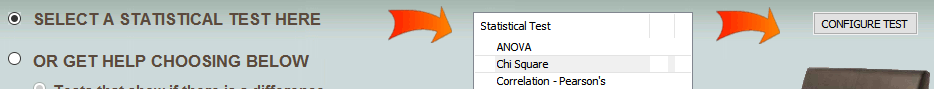
\includegraphics[width=0.95\linewidth]{gfx/cor055}}
      \caption{Starting Chi Square}
    \end{center}
  \end{figure}
  
  \item Data Source Table: email (It is desired to see if the correlation between the types of numbers in a message and the number of attachments is significant.)
  \item Group A: Number
  \item Group B: Image
  \item \texttt{SOFA} calculates the p-value of $ 0.01199 $, chi square of $ 19.593 $ and the degrees of freedom of $ 8 $.

  \begin{figure}[H]
    \begin{center}
      \fbox{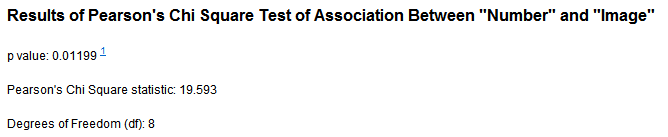
\includegraphics[width=0.95\linewidth]{gfx/cor060}}
      \caption{Chi Square Results}
    \end{center}
  \end{figure}

  \item Chi square results are normally printed in a matrix where the expected and actual values for each of the correlated variables are compared. 

  \begin{figure}[H]
    \begin{center}
      \fbox{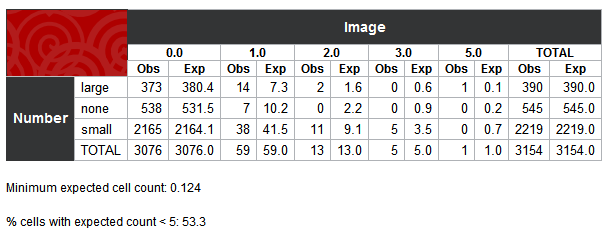
\includegraphics[width=0.95\linewidth]{gfx/cor065}}
      \caption{Chi Square Matrix}
      \label{cor:chi_square_matrix}
    \end{center}
  \end{figure}

  \item In the chi square matrix each level for both variables is calculated and compared. For example, in the matrix in Figure \ref{cor:chi_square_matrix}, ``Large'' numbers were observed $ 373 $ times and were expected $ 380.4 $ times. As long as the two values are close to each other then there is not much statistical significance in the values, in other words, the observed values are about what was expected. Under the matrix \texttt{SOFA} notes that the minimum expected cell count for the entire matrix is $ 0.124 $ and $ 53.3\% $ of the expected values are less than $ 5 $.

\end{enumerate}

\subsection{Activity 3: Chi Square} \label{cor:act03}

Using the \textit{maincafe} dataset in \texttt{SOFA}, determine Chi Square where Group A is Meal and Group B is Ptysize. Submit a screen capture from \texttt{SOFA} that shows the p value, Pearson's Chi Square statistic, Degrees of Freedom, the Ptysize Matrix, the Minimum expected cell count, and the percentage of cells with the expected count.

\section{Deliverable}

Complete the following activities in this lab:

\rowcolors{1}{gray!25}{}
\begin{center}
  \begin{tabular}{lll}
    \hline 
    \textbf{Number} & \textbf{Name} & \textbf{Page} \\ 
    \hline 
    \ref{cor:act01} & \nameref{cor:act01} & \pageref{cor:act01} \\ 
    \ref{cor:act02} & \nameref{cor:act02} & \pageref{cor:act02} \\ 
    \ref{cor:act03} & \nameref{cor:act03} & \pageref{cor:act03} \\ 
    \hline 
  \end{tabular} 
\end{center}

Consolidate the responses for all activities into a single document and submit that document for grading.

